

\documentclass{cv}


\geometry{left=6.0cm,top=2cm,right=1.5cm,bottom=0.7cm,nohead,nofoot}

\addbibresource{publis.bib} % Specify the bibliography file to include publications


\def\firstname{Benjamin}
\def\familyname{Vial}
\def\FileSubject{cover letter}
\def\FileAuthor{\firstname~\familyname}
\def\FileTitle{\firstname~\familyname's~\FileSubject}
\def\FileKeyWords{\firstname~\familyname, \FileSubject}

  \RequirePackage[unicode]{hyperref}% unicode is required for unicode pdf metadata
  \hypersetup{
    breaklinks,
    baseurl       = http://,
    pdfborder     = 0 0 0,
    pdfpagemode   = UseNone,% do not show thumbnails or bookmarks on opening
    pdfstartpage  = 1,
%    pdfproducer   = {\LaTeX{}},% will/should be set automatically to the correct TeX engine used
    bookmarksopen = true,
    bookmarksdepth= 2,% to show sections and subsections
    pdfauthor   = {\FileAuthor},%
    pdftitle    = {\FileTitle},%
    pdfsubject  = {\FileSubject},%
    pdfkeywords = {\FileKeyWords},%
    pdfcreator  = {\LaTeX},%
    pdfproducer = {\LaTeX}
    }


\begin{document}




\header{Benjamin}{~Vial}{Posdoctoral Research Asssistant | Wave Physics and Metamaterials}
\begin{tikzpicture}[remember picture, overlay]
	\node [anchor=north west, inner sep=0.3cm]  at (current page.north west)
	{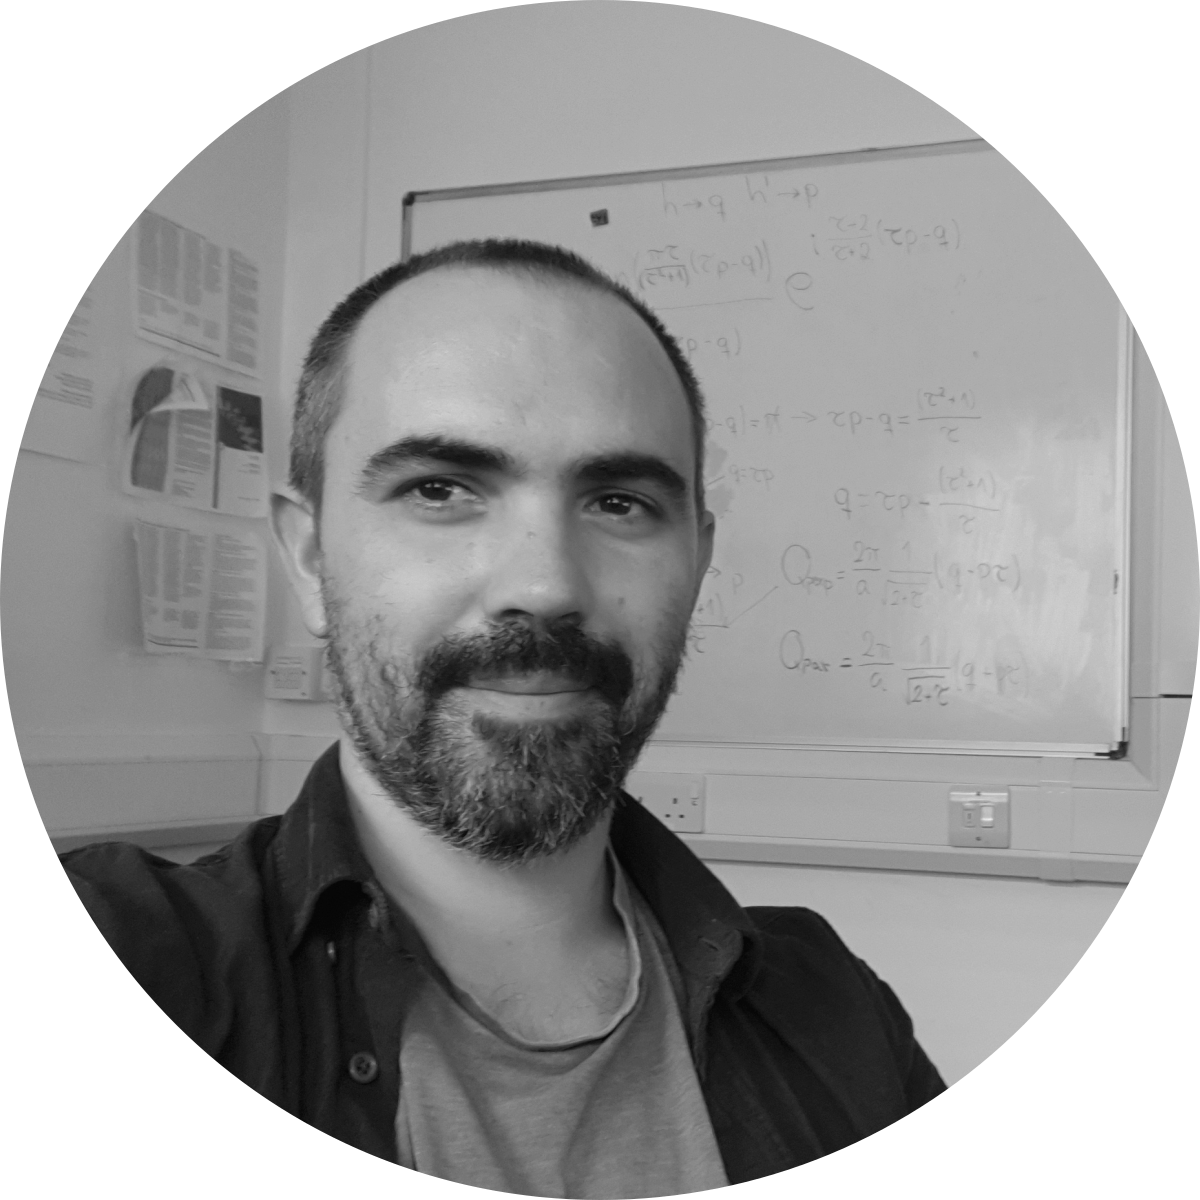
\includegraphics[height=3cm]{pic}};
\end{tikzpicture}
%----------------------------------------------------------------------------------------
%	SIDEBAR SECTION
%----------------------------------------------------------------------------------------

\begin{aside} % In the aside, each new line forces a line break
	\section{Contact}
	\faHome~~146 Glyn road
	London E5 0JE, UK
	\faPhone~~+44~7840~029~744
	\faEnvelope~~\href{mailto:b.vial@imperial.ac.uk}{b.vial@imperial.ac.uk}
	\faUser~~\href{http://bvial.info/}{bvial.info}
	\section{Information}
	date of birth 09/11/1984
	French citizenship
	\section{Languages}
	French mother tongue
	English fluent
	Spanish basic
	\section{Programming}
	\textbf{operating systems}
	Linux, Windows
	\textbf{languages and scripts}
	Python, Matlab, Mathematica, \LaTeX, C, C++, Q\#, HTML, CSS
	\textbf{applications}
	git, Comsol Multiphysics, Fenics, Gmsh, GetDP, Gimp, LibreOffice, Labview
	\section{Interests}
	\textbf{professional}
	Optics
	Photonics
	Metamaterials
	wave physics
	light-matter interraction
	homogenization methods
	computational EM
	numerical modelling
	optimization techniques
	inverse design
	finite element method
	Fourier modal method
	modal analysis
	machine learning
	Transformation Optics
	invisibility cloaking
	fabrication
	characterization
	open source science
	\textbf{personal}
	playing the guitar
	listening to music
	football, snowboard, hiking
	traveling, cooking
\end{aside}


%----------------------------------------------------------------------------------------
%	EDUCATION SECTION
%----------------------------------------------------------------------------------------

\section{Education}

\begin{entrylist}
	%------------------------------------------------
	\entry
	{Apr. 2013}
	{PhD {\normalfont in Physics}}
	{\href{http://www.fresnel.fr/}{Institut Fresnel}, CNRS, Centrale Marseille, Aix Marseille Universit\'e, Marseille, France}
	{Optics, Photonics and image processing}
	%------------------------------------------------
	\entry
	{Oct. 2009}
	{Master's degree {\normalfont in Physics}}
	{\href{http://www.centrale-marseille.fr/}{~~Centrale Marseille}~/~
		\href{http://www.lma.cnrs-mrs.fr/}{Laboratoire de Mécanique et d'Acoustique}, CNRS, Marseille, France}
	{Mechanics, Physics and Engineering, specialization in Acoustics}

	\entry
	{Oct. 2009}
	{Master's degree {\normalfont in Engineering}}
	{\href{http://www.centrale-marseille.fr/}{Centrale Marseille}, Marseille, France}
	{High level scientific and technical training}
	%------------------------------------------------
\end{entrylist}

%----------------------------------------------------------------------------------------
%	WORK EXPERIENCE SECTION
%----------------------------------------------------------------------------------------
\vspace*{-0.2cm}
\section{Research activities}

\begin{entrylist}
	%------------------------------------------------


	\entry
	{Aug. 2022 \\Now}
	{Postdoctoral Research Assistant}
	{\href{http://imperial.ac.uk/}{Imperial College London}, London, UK}
	{\href{https://www.metaveh.com/}{Projet METAVEH}: energy harvesting with elastic metamaterials. Developing and optimizing models of discrete mechanical lattices and resonators on thin plates.
	}


	\entry
	{Jan. 2019 \\Jul. 2022}
	{Postdoctoral Research Assistant}
	{\href{http://antennas.eecs.qmul.ac.uk/}{Queen Mary, University of London}, London, UK}
	{\href{https://animate-research.com/}{ANIMATE project}: nonlinear coupling model, homogenization of ferroelectric metamaterials, inverse design for tunability enhancement, microwave and THz material characterization.
	}


	\entry
	{Jan. 2017 \\Dec. 2018}
	{Postdoctoral Research Assistant}
	{\href{http://antennas.eecs.qmul.ac.uk/}{Queen Mary, University of London}, London, UK}
	{AOTOMAT project : Optimization tools and machine learning for the design of electromagnetic
		devices and materials.
	}

	\entry
	{Jul. 2014 \\Dec. 2016}
	{Postdoctoral Research Assistant}
	{\href{http://antennas.eecs.qmul.ac.uk/}{Queen Mary, University of London}, London, UK}
	{\href{http://www.quest-spatial-transformation.org/}{QUEST project}
		Transformation Optics applied to the design, fabrication and characterization of novel electromagnetic devices using metamaterials.
		Development of simulation tools and optimization techniques.
	}


	\entry
	{Nov. 2013\\ Jan. 2014}
	{Postdoctoral Research Assistant}
	{\href{http://www.fresnel.fr/}{Institut Fresnel}, Marseille, France}
	{
		Numerical study of the coupling of light
		to subwavelength resonant optical antennas and control of the local density of states.
	}
	%------------------------------------------------
	\entry
	{May 2013 \\Oct. 2013}
	{Postdoctoral Research Assistant}
	{\href{http://www.fresnel.fr/}{Institut Fresnel}, Marseille, France}
	{
		Development of simulation tools for ray tracing in complex media, inverse problem of
		finding index distribution to make light follow a prescribed path, deshomogenization
		technique with graded index photonic crystals.
	}

	%------------------------------------------------
	\entry
	{Oct. 2009\\Apr. 2013}
	{PhD in Physics}
	{\href{http://www.fresnel.fr/}{Institut Fresnel}~--~\href{http://www.silios.com/}{Silios Technologies}, Marseille, France}
	{\emph{\href{http://tel.archives-ouvertes.fr/index.php?halsid=slas337fv1oqlj1okgkq7q42i5&view_this_doc=tel-00918651&version=1}
			{Study of open electromagnetic resonators by modal approach.
				Application to infrared multispectral filtering.}} (\emph{joint academia/industry funding})\\
		FEM modelling of metamaterials, spectral analysis quasi-normal mode expansion.
		Application to the design of infrared filters for multispectral imaging devices.
		Fabrication and characterization of reflexion bandcut and transmission bandpass filters.
	}

\end{entrylist}


\section{Awards and honours}

  {Best PhD thesis 2014 award} from the {\href{https://ecole-doctorale-352.univ-amu.fr/en}{Doctoral School 352, Physics and Condensed Matter Science}}

  {Best PhD thesis 2014 award from {\href{https://www.cnano-paca.fr/index.php?option=com_content&view=article&id=80}{CNano PACA}}, finalized research category}





\newpage


%----------------------------------------------------------------------------------------
%	Teaching/supervising experience SECTION
%----------------------------------------------------------------------------------------

\vspace*{-0.2cm}
\section{Teaching/supervising experience}

\begin{entrylist}

	\entry
	{feb. 2023 - sept. 2023}
	{PhD co-supervision}
	{Imperial College London, London, UK.}
	{Visiting student from  Politechnico di Milano.\\
		\emph{Isospectral open cavities and curvilinear homogenization.}}
	\entry
	{jul. 2023 - sept. 2023}
	{Summer project supervision}
	{Imperial College London, London, UK.}
	{Applied mathematics undergrad student, 3 months.\\
		\emph{Optimizing dispersion in discrete phononic lattices.}}

	\entry
	{sept. 2018 - apr. 2022}
	{PhD co-supervision}
	{Queen Mary University of London, London, UK.}
	{Work with 2 PhD students.\\
		\emph{Data-driven optimisation of metasurfaces.}}

	\entry
	{nov. 2019 - apr. 2020}
	{Teaching Assistant}
	{Queen Mary University of London, London, UK.}
	{Quantum Programming. Lectures and tutorials on quantum physics, gates and circuits.
		Coding laboratory and projects in Q\# and Python. Preparation and correction of exams. (10 Master students, 6 months) }


	\entry
	{nov. 2018 - apr. 2019}
	{Co-supervision undergraduate project}
	{Queen Mary University of London, London, UK.}
	{Multidisciplinary project, 4 students.\\
		\emph{Detecting emotions with physiological and microwaves measurements.}}
	\entry
	{may-june 2012}
	{Internship tutor}
	{Institut Fresnel, Marseille, France.}
	{Tutor for an internship, 3rd year student of École Centrale Marseille.\\
		\emph{Optimization of infrared diffractive filters for infrared imaging.}}
	\entry
	{jan.-feb. 2011}
	{Project tutor}
	{Institut Fresnel, Marseille, France.}
	{Tutor for final year project, 5 students, 2nd year in École Centrale Marseille.\\
		\emph{Design of high efficiency solar cells with metamaterials}}

\end{entrylist}


\section{Administrative experience}

\begin{entrylist}

	\entry
	{nov. 2023}
	{Workshop organization}
	{Imperial College London, London, UK.}
	{Meeting and workshop on two European projects. Invitations, logistics, catering, technical programme writing.}

	\entry
	{2017}
	{Seminars organization}
	{Queen Mary University of London, London, UK.}
	{Internal seminar of Antennas and Electromagnetics research group}

	\entry
	{2017-2018}
	{Grant projects writing}
	{Queen Mary University of London, London, UK.}
	{
		Help in writing 2 projects to obtain grants from EPSRC. Both (AOTOMAT et ANIMATE) got accepted.}

	\entry
	{Sept. 2018- Jul. 2022}
	{Project management}
	{Queen Mary University of London, London, UK.}
	{
		Management of the ANIMATE project: website creation, planning meetings,
		liaising with academic and industrial partners.}


\end{entrylist}

\newgeometry{left=1.5cm,top=1.8cm,right=1.5cm,bottom=0.7cm,nohead,nofoot}

%----------------------------------------------------------------------------------------
%	Referees contact SECTION
%----------------------------------------------------------------------------------------


% \section{References}

% Available on request.

% 
% \section{Referees contact}
% 
% \begin{minipage}{.6\textwidth}
% 	\textbf{Prof Yang Hao}\\
% 	\faHome~~School of Electronic Engineering and Computer Science\\
% 	Queen Mary University of London\\
% 	Peter Landin Building, 10 Godward Square, Mile End Road\\
% 	London E1 4FZ, United Kingdom\\
% 	\faEnvelope~~\href{mailto:y.hao@qmul.ac.uk}{y.hao@qmul.ac.uk}\\
% 	\faPhone~~+44 20 7882 5341\\
% 	\faUser~~\href{http://www.eecs.qmul.ac.uk/~yang/}{www.eecs.qmul.ac.uk/~yang/}
% \end{minipage}%
% \begin{minipage}{0.4\textwidth}
% 	\textbf{Prof Andr\'e Nicolet}\\
% 	\faHome~~Aix-Marseille Université\\
% 	Institut Fresnel (UMR CNRS 6133)\\
% 	Domaine Universitaire de Saint-Jérôme\\
% 	F13397 Marseille cedex 20, France\\
% 	\faEnvelope~~\href{mailto:andre.nicolet@fresnel.fr}{andre.nicolet@fresnel.fr}\\
% 	\faPhone~~+33 4 91 28 87 73\\
% 	\faUser~~\href{https://www.fresnel.fr/perso/nicolet/}{www.fresnel.fr/perso/nicolet/}
% \end{minipage}

\newpage

%----------------------------------------------------------------------------------------
%	Publications SECTION
%----------------------------------------------------------------------------------------


\section{Publications}

\nocite{*}

\newrefcontext[labelprefix=A]
\printbibliography[type=article, title={Articles in peer-reviewed journals}, keyword={ricl}, heading=subbibliography]

\newrefcontext[labelprefix=B]
\printbibliography[type=book, title={Contribution to book chapter}, keyword={book}, heading=subbibliography]

\newrefcontext[labelprefix=C]
\printbibliography[type=inproceedings, title={Proceedings of international peer-reviewed conferences}, keyword={lecture comittee}, heading=subbibliography]

\newrefcontext[labelprefix=D]
\printbibliography[type=inproceedings, title={International peer-reviewed conferences}, keyword={conference}, heading=subbibliography]

\newrefcontext[labelprefix=E]
\printbibliography[type=inproceedings, title={National conferences and seminars}, keyword={france}, heading=subbibliography]
\newrefcontext[labelprefix=F]
\printbibliography[type=thesis, title={PhD thesis}, keyword={these}, heading=subbibliography]
\newrefcontext[labelprefix=G]
\printbibliography[type=article, title={In preparation}, keyword={prep}, heading=subbibliography]
\newrefcontext[labelprefix=H]
\printbibliography[type=software, title={Open source software and codes}, keyword={code}, heading=subbibliography]



\end{document}
